% GENERATED by make_paper_assets.py -- do not edit by hand.
\begin{figure}[t]
\centering
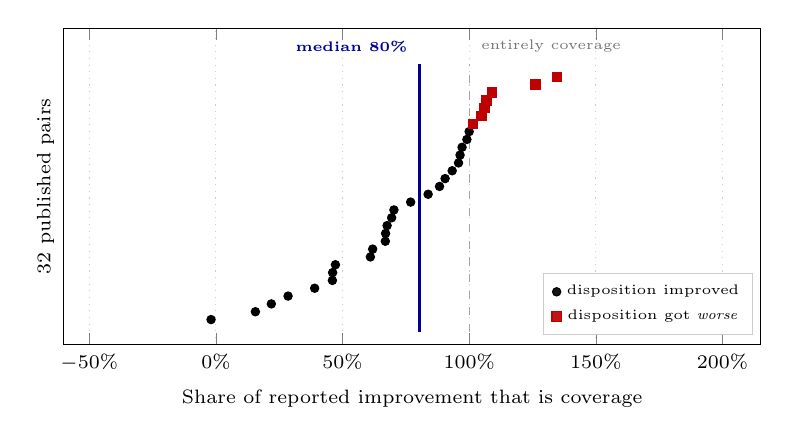
\begin{tikzpicture}
\begin{axis}[
  width=0.86\columnwidth, height=5.6cm,
  xmin=-60, xmax=215, ymin=-3.2, ymax=37.2,
  xtick={-50,0,50,100,150,200},
  xticklabels={$-$50\%,0\%,50\%,100\%,150\%,200\%},
  ytick=\empty,
  xlabel={Share of reported improvement that is coverage},
  ylabel={32 published pairs},
  tick label style={font=\scriptsize}, label style={font=\scriptsize},
  xmajorgrids, grid style={dotted, gray!40},
  legend style={at={(0.99,0.03)}, anchor=south east, font=\tiny,
                draw=gray!40, fill=white, fill opacity=0.92, text opacity=1},
  clip=false,
]
\draw[dashed, gray!70] (axis cs:100,-1.6) -- (axis cs:100,32.6);
\node[anchor=south west, font=\tiny, gray!90!black] at
  (axis cs:101,32.9) {entirely coverage};
\draw[thick, blue!60!black] (axis cs:80.4,-1.6) --
  (axis cs:80.4,32.6);
\node[anchor=south east, font=\tiny\bfseries, blue!60!black] at
  (axis cs:79.4,32.9) {median 80\%};
\addplot[only marks, mark=*, mark size=1.5pt, black]
  coordinates {(-1.9,0) (15.6,1) (21.9,2) (28.5,3) (39.0,4) (46.0,5) (46.1,6) (47.2,7) (61.0,8) (61.9,9) (66.9,10) (67.0,11) (67.6,12) (69.4,13) (70.3,14) (76.9,15) (83.8,16) (88.3,17) (90.5,18) (93.3,19) (95.8,20) (96.4,21) (97.2,22) (99.1,23) (100.0,24)};
\addlegendentry{disposition improved}
\addplot[only marks, mark=square*, mark size=1.7pt, red!75!black]
  coordinates {(101.6,25) (104.8,26) (106.0,27) (106.9,28) (109.0,29) (126.1,30) (134.6,31)};
\addlegendentry{disposition got \emph{worse}}
\end{axis}
\end{tikzpicture}
\caption{Every method--model pair in \citet{bae2025decap}'s ambiguous-split
table, sorted by the share of its reported bias-score improvement that is
coverage (the model abstaining more) rather than disposition (the model
actually preferring the stereotype less). Points beyond 100\% are pairs where
coverage over-explains the reported gain because disposition moved the wrong
way. The seven squares are pairs whose committed-answer bias \emph{worsened}
while the reported score improved.}
\label{fig:decomposition}
\end{figure}
